\section{Sistema coordenado cartesiano.}
Los factores de escala son:
\begin{align}
\begin{aligned}
h_{1} &=& h_{x} = 1 \\
h_{2} &=& h_{y} = 1 \\
h_{3} &=& h_{z} = 1 \\
\end{aligned}
\end{align}
Las familias de superficies coordenadas son tres conjuntos de planos paralelos $x=$ constante, $y=$ constante y $z=$ constantes. El sistema coordenado cartesiano es único en cuanto que todas las $h_{i}$ son constantes. Esto representará una ventaja considerable en el tratamiento de los tensores. Los vectores unitarios $\vu{i}, \vu{j}, \vu{k}$, tienen direcciones fijas.
\par
Las siguientes expresiones corresponden para el gradiente, divergencia, laplaciano y rotacional:
\begin{align}
\grad{\psi} &= \vu{i} \pdv{\psi}{x} + \vb{j} \pdv{\psi}{y} + \vu{k} \pdv{\psi}{z} \\[1em]
\div{\vb{V}} &= \pdv{\psi}{x} + \pdv{\psi}{y} + \pdv{\psi}{z} \\[1em]
\grad \cdot \grad{\psi} &= \pdv[2]{\psi}{x} + \pdv[2]{\psi}{y} +  \pdv[2]{\psi}{z} \\[1em]
\curl{\vb{V}} &= \mdet{
\vu{i} & \vu{j} & \vu{k} \\[0.5em]
\displaystyle \pdv{x} & \displaystyle \pdv{y} & \displaystyle \pdv{z} \\[0.5em]
V_{x} & V_{y} & V_{z}
}
\end{align}

\section{Sistema coordenado cilíndrico \texorpdfstring{$(\rho, \varphi, z)$}{(r, t, z)}}

En el sistema coordenado cilíndrico las tres coordenadas curvilíneas del sistema generalizado $(q_{1}, q_{2}, q_{3})$, se renombran por $(\rho, \varphi, z)$. Usamos $\rho$ para la distancia perpendicular desde el eje $z$ y dejando $r$ para la distancia desde el origen. Los límites de $\rho, \varphi$ y $z$, son:
\begin{align*}
0 \leq \rho < \infty, \hspace{1cm} 0 \leq \varphi \leq 2 \pi, \hspace{1cm} -\infty < z < \infty
\end{align*}
Las superficies coordenadas las podemos ver en la figura (\ref{fig:figura_sistema_01_cilindrico}):
\begin{enumerate}
\item Los cilindros circulares tienen al eje $z$ como eje común, tal que:
\begin{align*}
\rho =  (x^{2} + y^{2})^{1/2} = \text{constante}
\end{align*}
\item Los semiplanos a través del eje $z$
\begin{align*}
\varphi = \tan^{-1} \left(\dfrac{y}{x} \right) = \text{constante}
\end{align*}
\item Los planos paralelos al plano $x-y$, como en el sistema cartesiano:
\begin{align*}
z = \text{constante}
\end{align*}
\end{enumerate}
\begin{figure}[H]
    \centering
    % \tdplotsetmaincoords{70}{120}
    % \begin{tikzpicture}[tdplot_main_coords][scale=0.75]
    % \tikzstyle{every node}=[font=\small]
    % \draw[thick,-latex] (0,0,0) -- (6,0,0) node[anchor=north east]{$x$};
    % \draw[thick,-latex] (0,0,0) -- (0,6,0) node[anchor=north west]{$y$};
    % \draw[thick,-latex] (0,0,0) -- (0,0,6) node[anchor=south]{$z$};
    % \draw [thick](0,0,0) circle (3);
    % \draw [thick](0,0,4) circle (3);
    % \draw [thick](1.9,-2.35,0) -- (1.9,-2.35,4) node[midway, left]{$\rho=\rho_1$ superficie};
    % \draw [thick](-1.9,2.35,0) -- (-1.9,2.35,4);
    % \filldraw[fill=orange, nearly transparent] (-4,-4,4) -- (4,-4,4) --  (4,5,4) -- (-4,5,4) -- (-4,-4,4);
    % \filldraw[fill=blue, nearly transparent] (0,0,4) -- (5.2,6,4) --  (5.2,6,0) -- (0,0,0) -- (0,0,4);
    % \filldraw [color=blue](2,2.25,4) circle (0.075cm) ;
    % \draw (-4,5,4) node[anchor=south]{$z=z_1$ plano};
    % \draw (5.2,6,0) node[anchor=south west]{$\varphi=\varphi_1$ plano};
    % \node at (1.8,1,4)  { $\rho_{1}(\rho_{1},\varphi_{1},z_{1})$};
    % \draw[ultra thick,-latex](2,2.25,4) -- (3,3.45,4) node[anchor=north] {$\bm{\rho}_{0}$};
    % \draw[ultra thick,-latex](2,2.25,4) -- (1,2.5,4) node[anchor=north west] {$\bm{\varphi}_{0}$};
    % \draw[ultra thick,-latex](2,2.25,4) -- (2,2.25,4.75) node[anchor=north west] {$\mathbf{k}$};
    % \draw [thick,->](4,0,0) arc (0:45:4 and 4.5);
    % \draw (3.6,2,0) node[anchor=north] {$\varphi_1$};
    % \draw[ultra thick,-latex](0,0,0) -- (2,2.35,0);
    % \draw (1,1,0) node[anchor=north] {$\rho_1$};
    % \draw [ultra thick] (2,2.25,4)--(1.95,2.25,0);
    % \draw[ultra thick](0.1,0,4) -- (-0.1,0,4) node[anchor=south west] {$z_1$};
    % \end{tikzpicture}
    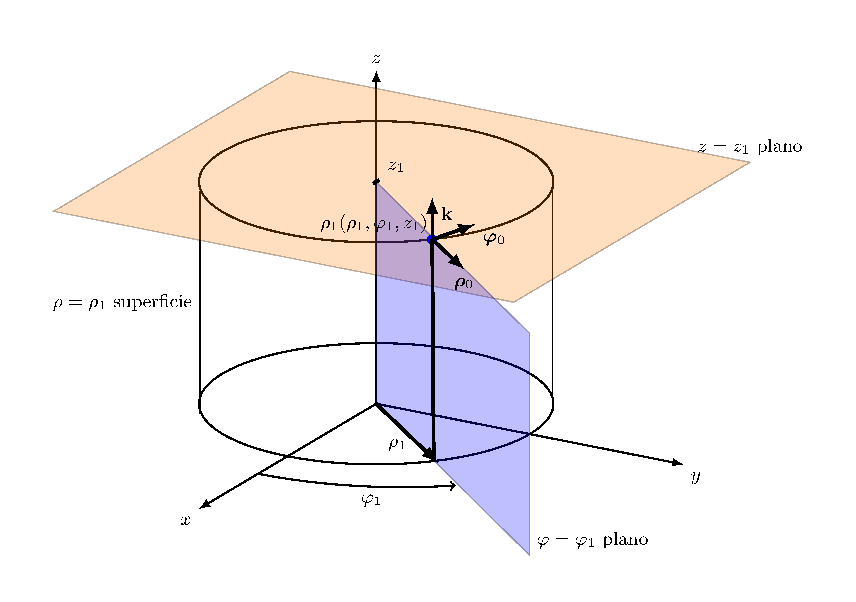
\includegraphics[scale=1]{Imagenes/Sistema_Cilindrico_01.eps}
    \caption{Sistema coordenado cilíndrico.}
    \label{fig:figura_sistema_01_cilindrico}
\end{figure}
Podemos recuperar las relaciones de transformación:
\begin{align}
\begin{aligned}
x &= \rho \, \cos \varphi \\
y &= \rho \, \sin \varphi \\
z &= z
\end{aligned}
\label{eq:ecuacion_02_028}
\end{align}
Considerando los elementos de longitud $\dd{s_{1}}$, encontramos que los factores de escala son:
\begin{align}
\begin{aligned}
h_{1} &= h_{\rho} = 1 \\
h_{2} &= h_{\varphi} = \rho \\
h_{3} &= h_{z} = 1
\end{aligned}
\label{eq:ecuacion_02_029}
\end{align}
Los vectores unitarios $(\vu{q}_{1},\vu{q}_{2},\vu{q}_{3})$ se renombran $(\vu*{\rho},\vu*{\varphi},\vu*{z})$:
\begin{enumerate}
\item El vector unitario $\vu*{\rho}$ es normal a la superficie cilíndrica que apunta en la dirección del incremento del radio $\rho$.
\item El vector unitario $\vu*{\varphi}$ es tangencial a la superficie cilíndrica y además, perpendicular al semiplano $\varphi=\text{constante}$, y el vector apunta en la dirección del incremento del ángulo azimutal $\varphi$.
\item El vector $\vu*{z}$, es el vector unitario que conocemos del sistema cartesiano.
\end{enumerate}
Estos vectores son mutuamente ortogonales
\begin{align*}
\vu*{\rho} \cdot \vu*{\varphi} = \vu*{\varphi} \cdot \vu*{z} = \vu*{z} \cdot \vu*{\rho} = 0
\end{align*}
un vector coordenado y un vector general $\mathbf{V}$ se expresan por
\begin{align*}
\vb{r} &= \vu*{\rho} \, \rho + \vu*{z} \, z \\
\vb{V} &=  \vu*{\rho} \, V_{\rho} + \vu*{\varphi} \, V_{\varphi} + \vu*{z} \, V_{z}
\end{align*}
Un elemento diferencial de desplazamiento $d \mathbf{r}$ se puede escribir como
\begin{align}
\begin{aligned}
\dd{\vb{r}} &= \vu*{\rho} \dd{s_{\rho}} + \vu*{\varphi}  \dd{s_{\varphi}} + \vu*{z} \dd{z} \\
&= \vu*{\rho} \dd{\rho} + \vu*{\varphi} \: \rho \dd{\varphi} + \vu*{z} \dd{z}
\end{aligned}
\end{align}
Los operadores diferenciales que involucran al operador $\grad$, resultan ser:
\begin{align}
\grad{\psi} (\rho, \varphi, z) &= \vu*{\rho} \, \pdv{\psi}{\rho} + \vu*{\varphi} \, \dfrac{1}{\rho} \, \pdv{\psi}{\varphi} + \vu*{z} \pdv{\psi}{z} \label{eq:ecuacion_02_033}\\[1em]
\div{V} &= \dfrac{1}{\rho} \, \pdv{\rho} (\rho \, V_{\rho}) + \dfrac{1}{\rho} \, \pdv{V_{\varphi}}{\varphi} + \pdv{V_{z}}{z} \label{eq:ecuacion_02_034} \\[1em]
\laplacian{\psi} &= \dfrac{1}{\rho} \, \pdv{\rho} \left( \rho \, \pdv{\psi}{\rho} \right) + \dfrac{1}{\rho^{2}} \, \pdv[2]{\psi}{\varphi} + \pdv[2]{\psi}{z} \label{eq:ecuacion_02_035} \\[1em]
\curl{\vb{V}} &= \dfrac{1}{\rho} \, \renewcommand\arraystretch{1.5}
\mdet{
\vu*{\rho} & \rho \, \vu*{\varphi} & \vu*{z} \\
\displaystyle \pdv{\rho} & \displaystyle \pdv{\varphi} & \displaystyle \pdv{z} \\
V_{\rho} & \rho \, V_{\varphi} & V_{z}
}
\label{eq:ecuacion_02_036}
\end{align}
\\
\textbf{Ejemplo: } Las ecuaciones de Navier Stokes de la hidrodinámica incluyen un término no lineal:
\begin{align*}
\curl [ \vb{v} \cp ( \curl{\vb{v}})]
\end{align*}
donde $\vb{v}$ es la velocidad del fluido. Para flujos a través de un tubo cilíndrico en la dirección $z$
\begin{align*}
\vb{v} =  \vu*{z}  \, v (\rho)
\end{align*}
Calculamos primeramente el rotacional
\begin{align*}
\curl{\vb{v}} = \dfrac{1}{\rho} \, 
\renewcommand\arraystretch{1.5} \mdet{
\vu*{\rho} & \rho \, \vu*{\varphi} & \vu*{z} \\
\displaystyle \pdv{\rho} & \displaystyle \pdv{\varphi} & \displaystyle \pdv{z} \\
0 & 0 & v(\rho)
}
= - \vu*{\varphi} \, \pdv{v}{\rho}
\end{align*}
ahora calculamos el doble producto escalar (vector con vector)
\begin{align*}
\vb{v} \cp (\curl{\vb{v}}) =  
\renewcommand\arraystretch{1.5} \mdet{
\vu*{\rho} & \vu*{\varphi} & \vu*{z} \\
0 & 0 & v \\
0 & \displaystyle - \pdv{v}{\rho} & 0
}
= - \vu*{\rho} \, v(\rho) \, \pdv{v}{\rho} 
\end{align*} 
finalmente, el triple producto escalar resulta ser
\begin{align*}
\curl ( \vb{v} \cp (\curl{\vb{v}})) = \dfrac{1}{\rho} \, 
\renewcommand\arraystretch{1.75} \mdet{
\vu*{\rho} & \rho \, \vu*{\varphi} & \vu*{z} \\
\displaystyle \pdv{\rho} & \displaystyle \pdv{\varphi} & \displaystyle \pdv{z} \\
v \, \displaystyle \pdv{v}{\rho} & 0 & 0
}
= 0
\end{align*}
Para este caso en particular, los términos no lineales se anulan.

\section{Coordenadas esféricas polares \texorpdfstring{$(r, \theta, \varphi)$}{(r, t, v)}}

Las ecuaciones de transformación son:
\begin{align}
\begin{aligned}
x &= r \, \sin \theta \, \cos \varphi \\
y &= r \, \sin \theta \, \sin \varphi \\
z &= r \, \cos \theta
\end{aligned}
\label{eq:ecuacion_02_038}
\end{align}
Midiendo $\theta$ en el cuadrante positivo del eje $z$ positivo y $\varphi$ en el plano $x-y$ sobre el eje $x$ positivo. Los rangos donde varían las coordenadas son
\begin{align*}
0 \leq r < \infty \hspace{1.5cm} 0 \leq \theta \leq \pi \hspace{1.5cm} 0 \leq \varphi \leq 2 \pi
\end{align*}
Renombrando las coordenadas $(q_{1}, q_{2}, q_{3})$ como $(r, \theta, \varphi)$, vemos que el sistema coordenado esférico es consistente con:
\begin{enumerate}
\item Tenemos esferas concéntricas en el origen:
\begin{align*}
r = (x^{2} + y^{2} + z^{2})^{1/2} =  \text{constante}
\end{align*}
\item Hay conos circulares concéntricos en el eje $z$-polar, con vértices en el origen:
\begin{align*}
\theta = \arccos \dfrac{z}{(x^{2} +y^{2} + z^{2})^{1/2}} = \text{constante}
\end{align*}
\item Tenemos que los semiplanos pasan a través del eje $z$-polar:
\begin{align*}
\varphi = \arctan\left(\dfrac{y}{x} \right) =  \text{constante}
\end{align*}
\end{enumerate}
%\begin{center}
%\begin{figure}
%\begin{tikzpicture}
%\draw [dashed] (0,0) arc (180:0:4 and 2) ;
%\draw (0,0) arc (180:360:4 and 2) ;
%\draw [dashed] (0,0.5) arc (180:0:3.95 and 2) ;
%\draw (0,0.5) arc (180:360:3.95 and 2) ;
%\draw (0,0) arc (180:0:4 and 4);
%\end{tikzpicture}
%\end{figure}
%\end{center}
\begin{figure}
    \centering
    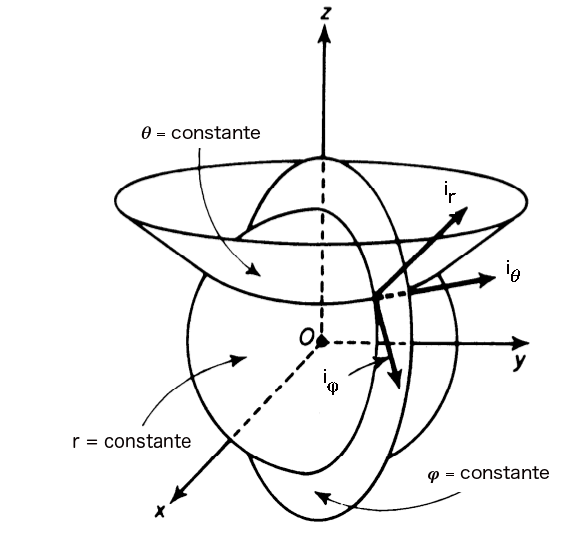
\includegraphics[scale=0.5]{Imagenes/CoordenadasEsfericasSuperficiesConstantes.png}
    \caption{Intersección de superficies constantes en el sistema coordenado esférico.}
    \label{fig:figura_coordenadas_esfericas_superficies}
\end{figure}
De acuerdo con nuestra selección arbitraria de definiciones para el ángulo polar $\theta$, y el ángulo azimutal $\varphi$, el eje $z$ es el elegido para un manejo especial. \begin{figure}[H]
    \centering
    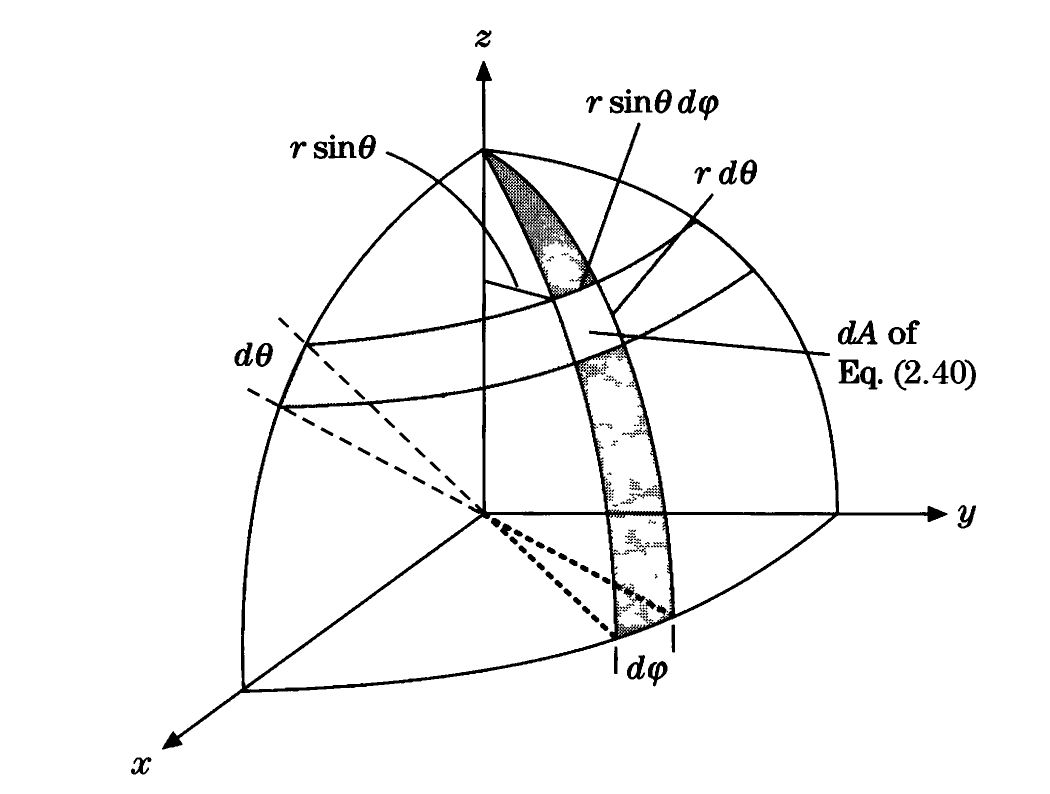
\includegraphics[scale=0.35]{Imagenes/Elemento_Area_Esferico}
    \caption{Elemento de área en el sistema coordenado esférico.}
    \label{fig:figura_elemento_area_esferico}
\end{figure}
Diferenciando las expresiones inversas, tenemos que 
\begin{align}
\begin{aligned}
h_{1} &= h_{r} = 1 \\
h_{2} &= h_{\theta} = r \\
h_{3} &= h_{\varphi} = r \, \sin \theta 
\end{aligned}
\label{eq:ecuacion_02_039}
\end{align}
Lo que nos da un elemento de línea
\begin{align*}
\dd{\vb{r}} = \vu*{r} \dd{r} + \vu*{\theta} \, r \dd{\theta} + \vu{\varphi} \, r \, \sin \theta \dd{\varphi}
\end{align*}
por tanto
\begin{align*}
\dd{s^{2}} = \dd{\vb{r}} \cdot \dd{\vb{r}} =  \dd{r^{2}} + r^{2} \, \dd{\theta^{2}} + r^{2} \, \sin^{2} \theta \dd{\varphi^{2}}
\end{align*}
En este sistema coordenado esférico, el elemento de área (para $r=\text{constante}$) es:
\begin{align*}
\dd{A} = \dd{\sigma_{\theta \varphi}} = r^{2} \, \sin \theta \dd{\theta} \dd{\varphi}
\end{align*}
Que corresponde al área sin sombra en la figura (\ref{fig:figura_elemento_area_esferico}).
\par
Integrando sobre la coordenada azimutal $\varphi$, se tiene que el elemento de área, genera un anillo de ancho $\dd{{\theta}}$
\begin{align*}
\dd{A_{\theta}} = 2 \, \pi \, r^{2} \sin \theta \dd{\theta}
\end{align*}
Esta expresión se presenta frecuentemente en problemas con coordenadas esféricas polares con simetría azimutal, tales como la dispersión de un haz no polarizado de partículas nucleares.
\par
Por definición de estereoradianes, un elemento de ángulo sólido $\dd{\Omega}$ está dado por:
\begin{align*}
\dd{\Omega} = \dfrac{\dd{A}}{r^{2}} = \sin \theta \dd{\theta} \dd{\varphi}
\end{align*}
Integrando sobre toda la superficie esférica, se obtiene
\begin{align*}
\int \dd{\Omega} = 4 \, \pi
\end{align*}
El elemento de volumen es:
\begin{align}
\begin{aligned}
\dd{\tau} &= r^{2} \dd{r} \, \sin \theta \dd{\theta} \dd{\varphi} \\
&= r^{2} \dd{r} \dd{\Omega}
\end{aligned}
\label{eq:ecuacion_02_043}
\end{align}
Los vectores unitarios del sistema polar esféricos se muestran en la siguiente figura (\ref{fig:figura_coordenadas_esfericas_vu}):
\begin{figure}[H]
    \centering
    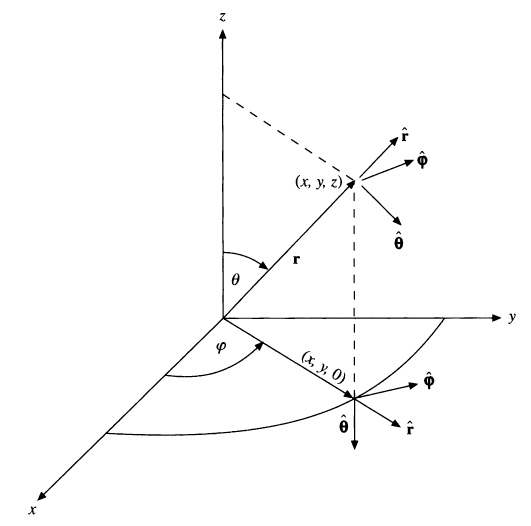
\includegraphics[scale=0.5]{Imagenes/CoordenadasEsfericasVectoresUnitarios.png}
    \caption{Coordenadas polares esféricas.}
    \label{fig:figura_coordenadas_esfericas_vu}
\end{figure}
%\begin{figure}[!h]
%\centering
%\tdplotsetmaincoords{60}{110}
%%
%\pgfmathsetmacro{\rvec}{.8}
%\pgfmathsetmacro{\thetavec}{30}
%\pgfmathsetmacro{\phivec}{60}
%%
%\begin{tikzpicture}[scale=5,tdplot_main_coords]
%    \coordinate (O) at (0,0,0);
%    \draw[thick,->] (0,0,0) -- (1,0,0) node[anchor=north east]{$x$};
%    \draw[thick,->] (0,0,0) -- (0,1,0) node[anchor=north west]{$y$};
%	\draw[thick,->] (0,0,0) -- (0,0,1) node[anchor=south]{$z$};
%    \tdplotsetcoord{P}{\rvec}{\thetavec}{\phivec}
%    \draw[-stealth,color=red] (O) -- (P) node[above right] {$P$};
%    \draw[dashed, color=red] (O) -- (Pxy);
%    \draw[dashed, color=red] (P) -- (Pxy);
%    %\draw[dashed, color=red] (0,0,0.7) -- (O);
%    \tdplotdrawarc{(O)}{0.4}{0}{\phivec}{anchor=north}{$\phi$}
%    \tdplotsetthetaplanecoords{\phivec}
%    \tdplotdrawarc[tdplot_rotated_coords]{(0,0,0)}{0.5}{0}%
%        {\thetavec}{anchor=south west}{$\theta$}
%
%
%\end{tikzpicture}
%\end{figure}
Se insiste en que los vectores unitarios $\vu*{r}, \vu*{\theta}, \vu*{\varphi}$ cambian de dirección conforme cambian los ángulos $\theta$ y $\varphi$. En términos de los vectores unitarios cartesianos $(\vu{i}, \vu{j}, \vu{k})$ cuya dirección es fija, tenemos que
\begin{align}
\begin{aligned}
\vu*{r} &= \vu{x} \, \sin \theta \, \cos \varphi + \vu{y} \, \sin \theta \, \sin \varphi + \vu{z} \, \cos \theta \\
\vu*{\theta} &= \vu{x} \, \cos \theta \, \cos \varphi + \vu{y} \, \cos \theta \, \sin \varphi - \vu{z} \, \sin \theta = \pdv{\vu{r}}{\theta} \\
\vu*{\varphi} &= - \vu{x} \, \sin \varphi + \vu{y} \, \cos \varphi = \dfrac{1}{\sin \theta} \pdv{\vu{r}}{\varphi}
\end{aligned}
\label{eq:ecuacion_02_044}
\end{align}
Dadas la transformación inversa y un vector dado, se puede expresar de diferentes maneras, por ejemplo el vector de posición $\vb{r}$ puede escribirse como
\begin{align}
\vb{r} &= \vu*{r} \, r = \vu*{r} \left( x^{2} + y^{2} + z^{2} \right)^{1/2} \nonumber \\
&= \vu{x} \, x + \vu{y} \, y + \vu{z} \, z \nonumber \\
&= \vu{x} \, r \, \sin \theta \, \cos \varphi + \vu{y} \, r \, \sin \theta \, \sin \varphi + \vu{z} \, r \, \cos \theta \label{eq:ecuacion_02_045}
\end{align}
De acuerdo al problema que se nos presente, para resolverlo debemos de elegir la expresión más útil.
\par
Renombrando los vectores unitarios del sistema de coordenadas curvilineas $(\vu{q}_{1}, \vu{q}_{2}, \vu{q}_{3}) $ como $(\vu*{r}, \vu*{\theta}, \vu*{\varphi})$, los operadores diferenciales son:
\begin{align}
\grad{\psi} &= \vu*{r} \pdv{\psi}{r} + \vu*{\theta} \, \dfrac{1}{r} \, \pdv{\psi}{\theta} + \vu*{\varphi} \, \dfrac{1}{r \, \sin \theta} \pdv{\psi}{\varphi} \label{eq:ecuacion_02_046} \\[1em]
\div{V} &= \dfrac{1}{r^{2} \sin \theta} \left[ \sin \theta \pdv{r}(r^{2} \, V_{r}) + r \, \pdv{\theta} (\sin \theta \, V_{\theta}) + r \, \pdv{V_{\varphi}}{\varphi} \right] \label{eq:ecuacion_02_047} \\[1em]
\grad \cdot \grad{\psi} &= \dfrac{1}{r^{2} \, \sin \theta} \left[  \sin \theta \, \pdv{r} \left( r^{2} \, \pdv{\psi}{r} \right) + \pdv{\theta} \left( \sin \theta \, \pdv{\psi}{\theta} \right) + \dfrac{1}{\sin \theta} \pdv[2]{\psi}{\varphi} \right] \label{eq:ecuacion_02_048} \\[1em]
\curl{V} &= \dfrac{1}{r^{2} \, \sin \theta}
\renewcommand\arraystretch{1.5} \mdet{
\vu*{r} & r \, \vu*{\theta} & r \, \sin \theta \, \vu*{\varphi} \\
\displaystyle \pdv{r} & \displaystyle \pdv{\theta} & \displaystyle \pdv{\varphi} \\
V_{r} & r \, V_{\theta} & r \, \sin \theta \, V_{\varphi}
}
\end{align}
\textbf{Ejercicio a cuenta:} Una partícula se mueve a través del espacio. Demuestra que las componentes en coordenadas esféricas de su velocidad y aceleración son:
\begin{align*}
\begin{aligned}
v_{r} &= \dot{r} \\
v_{\theta} &= r \, \dot{\theta} \\
v_{\varphi} &= r \, sin \theta \, \dot{\varphi}
\end{aligned}
\hspace{2cm}
\begin{aligned}
a_{r} &= \ddot{r} - r \, \dot{\theta}^{2} - r \, \sin^{2} \theta \, \dot{\varphi}^{2} \\
a_{\theta} &= r \, \ddot{\theta} + 2 \, \dot{r} \, \dot{\theta} - r \, \sin \theta \, \cos \theta \, \dot{\varphi}^{2} \\
a_{\varphi} &= r \, \sin \theta \, \ddot{\varphi} +  2 \, \dot{r} \, \sin \theta \, \dot{\varphi} + 2 \, r \, \cos \theta \, \dot{\theta} \, \dot{\varphi}
\end{aligned}
\end{align*}
\underline{Sugerencia:} Considera
\begin{align*}
\vb{r} = \vu*{r} (t) \, r(t) = [ \vu{x} \, \sin \theta (t)  \, \cos \varphi (t) + \vu{y} \, \sin \theta (t)  \, \sin \varphi (t) + \vu{z} \, \cos \theta (t) ] \, r(t)
\end{align*}
Utilizando las técnicas de Lagrange, estos resultados pueden obtenerse en una forma más elegante. La notación $\dot{r}, \dot{\theta}, \dot{\varphi}$ significa la derivada con respecto al tiempo $\dot{r} = \dv*{r}{t}$, $\dot{\theta} = \dv*{\theta}{t}$ y $\dot{\varphi} = \dv*{\varphi}{t}$.

\section{Construcción de sistemas coordenados.}



Para construir un sistema de coordenadas en un espacio euclidiano basta contar con una familia de curvas planas, definida en forma tal que a cada valor de un parámetro le corresponda una curva. La teoría vista nos permite construir una familia de curvas ortogonales a la familia original. Consideremos primero los sistemas coordenados en el orden de sus propiedades de simetría, como aquellos que tienen un eje de traslación. Todos esos sistemas coordenados que tiene un eje de translación son esencialmente sistemas bidimensionales con una tercera dimensión adjunta: el eje $z$.
 %De este modo se obtiene un sistema de coordenadas curvilíneas ortogonales en el plano. Por rotación o adición del eje $z$ pueden generarse sistemas coordenados en 3D. Así, las coordenadas cilíndricas y esféricas pueden ser obtenidas de las coordenadas polares incluyendo el eje $z$ o rotando alrededor del eje $y$.

 \subsection{Coordenadas cilíndricas elípticas \texorpdfstring{$(u, v, z)$}{(u, v, z)}.}
 
 Para el sistema cilíndrico elíptico, se tienen las siguientes reglas de transformación:
\begin{align}
\begin{aligned}
x &= a \, \cosh u \, \cos v \\
y &= a \, \sinh u \, \sin v \\
z &= z
\end{aligned}
\label{eq:ecuacion_02_73_esp}
\end{align}
Para identificar las superficies constantes, elevamos al cuadrado cada lado
\begin{align}
x^{2} &= a^{2} \, \cosh^{2} u \, \cos^{2} v \label{eq:ecuacion_02_74_esp} \\
y^{2} &= a^{2} \, \sinh^{2} u \, \sin^{2} v \label{eq:ecuacion_02_75_esp} \\ 
\end{align}
Dividimos la primera expresión entre $\cos^{2} v$ y la segunda entre $\sin^{2} v$, recordando que $cos^{2} + \sin^{2} = 1$, así llegamos a
\begin{align}
\dfrac{x^{2}}{a^{2} \, \cosh^{2}} + \dfrac{y^{2}}{a^{2} \, \sinh{2}} &= \cos^{2} + \sin^{2} = 1 \label{eq:ecuacion_02_76_esp}\\[1em]
\dfrac{x^{2}}{a^{2} \, \cos^{2}} - \dfrac{y^{2}}{a^{2} \, \sin^{2}} &= \cosh^{2} - \sinh^{2} = 1 \label{eq:ecuacion_02_77_esp}
\end{align}
Para $v=$ constante, la ec. (\ref{eq:ecuacion_02_76_esp}) genera una familia de elipses con el eje $x$, en el principal. Para $u=$ constante, la ec. (\ref{eq:ecuacion_02_77_esp}) genera hipérbolas con puntos focales en el eje $x$.
\begin{figure}[H]
    \centering
    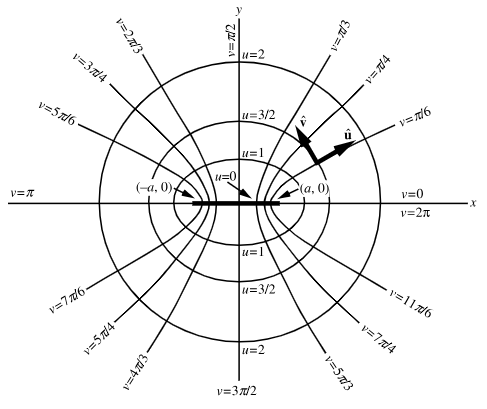
\includegraphics[scale=0.75]{Imagenes/EllipticCylindricalCoord_1000.png}
    \caption{Sistema coordenado cilíndirco elíptico en el plano $x-y$.}
    \label{fig:figura_coordenada_cilindricas_elipticas}
\end{figure}
La familia de superficies coordenadas son las siguientes:
\begin{enumerate}
\item Cilindros elípticos con $u$ constante, $0 \leq u < \infty$
\item Cilindros hiperbólicos conb $v$ constante, $0 \leq v \leq 2 \, \pi$
\item Planos paralelos al plano $x-y$ con $z$ constante, $-\infty < z < \infty$
\end{enumerate}
\begin{figure}[H]
    \centering
    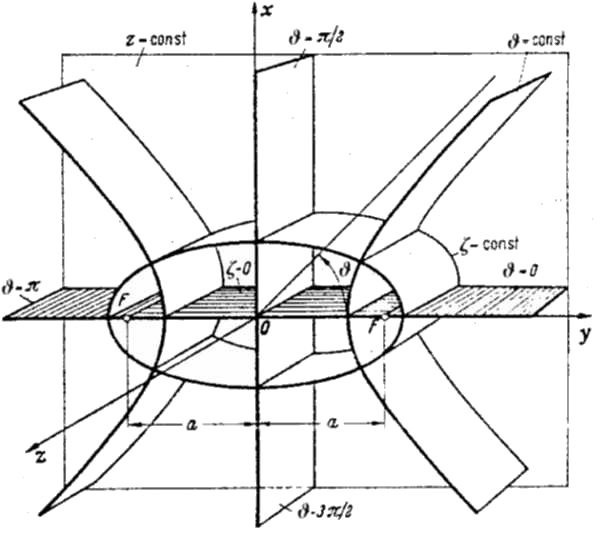
\includegraphics[scale=0.5]{Imagenes/Elliptic-cylindrical-coordinates_02.png}
    \caption{Sistema coordenado cilíndirco elíptico vista en tres dimensiones.}
    \label{fig:figura_coordenada_cilindricas_elipticas_3D}
\end{figure}
Calculamos los factores de escala o coeficientes métricos a partir de la expresión:
\begin{align*}
h_{i} = \sqrt{ \left( \pdv{x}{q_{i}} \right)^{2} + \left( \pdv{y}{q_{i}} \right)^{2} + \left( \pdv{z}{q_{i}} \right)^{2}}
\end{align*}
tenemos entonces que para $ i = u$
\begin{align*}
h_{1} = h_{u} = \sqrt{ \left( \pdv{x}{u} \right)^{2} + \left( \pdv{y}{u} \right)^{2} + \left( \pdv{z}{u} \right)^{2}}
\end{align*}
donde
\begin{align*}
\pdv{x}{u} &= a \, \sinh u \cos v \hspace{1cm} \Rightarrow \hspace{1cm} \left( \pdv{x}{u} \right)^{2} = a^{2} \, \sinh^{2} u \, \cos^{2} v \\[1em]
\pdv{y}{u} &= a \, \cosh u \sin v \hspace{1cm} \Rightarrow \hspace{1cm} \left( \pdv{y}{u} \right)^{2} = a^{2} \, \cosh^{2} u \, \sin^{2} v \\[1em]
\pdv{z}{u} &= 0
\end{align*}
al sumar los términos del radical
\begin{align*}
h_{u} = \sqrt{a^{2} \, \sinh^{2} u \, \cos^{2} v + a^{2} \, \cosh^{2} u \, \sin^{2} v}
\end{align*}
Haciendo el álgebra respectiva y considerando que $\cosh^{2} u - \sinh^{2} = 1$, entonces:
\begin{align*}
h_{u} &= \sqrt{a^{2} \left[ \sinh^{2} u \, \cos^{2} v + \cosh^{2} u \, \sin^{2} v \right] } \\[1em]
&= \sqrt{a^{2} \left[ \sinh^{2} u \, \cos^{2} v + (1 + \sinh^{2} u) \, \sin^{2} v \right] } \\[1em]
&= \sqrt{a^{2} \left[ \sinh^{2} u \, \cos^{2} v + \sinh^{2} u \, \sin^{2} v + \sin^{2} v \right] } \\[1em]
&= \sqrt{a^{2} \left[ \sinh^{2} u ( \cos^{2} v + \sin^{2}v ) + \sin^{2} v \right] } \\[1em]
&= \sqrt{a^{2} \left[ \sinh^{2} u + \sin^{2} v  \right] } \\[1em]
h_{u} &= a \, \sqrt{ \sinh^{2} u + \sin^{2} v}
\end{align*}
Para el factor $h_{v}$ se tiene que
\begin{align*}
h_{v} = \sqrt{ \left( \pdv{x}{v} \right)^{2} + \left( \pdv{y}{v} \right)^{2} + \left( \pdv{z}{v} \right)^{2}}
\end{align*}
entonces
\begin{align*}
\pdv{x}{v} &= - a \, \cosh u \sin v \hspace{1cm} \Rightarrow \hspace{1cm} \left( \pdv{x}{v} \right)^{2} = a^{2} \, \cosh^{2} u \, \sin^{2} v \\[1em]
\pdv{y}{v} &= a \, \sinh u \cos v \hspace{1cm} \Rightarrow \hspace{1cm} \left( \pdv{y}{v} \right)^{2} = a^{2} \, \sinh^{2} u \, \cos^{2} v \\[1em]
\pdv{z}{v} &= 0
\end{align*}
así llegamos a que
\begin{align*}
h_{v} &= \sqrt{a^{2} \left[ \cosh^{2} u \, \sin^{2} v + \sinh^{2} u \, \cos^{2} v \right] } \\[1em]
&= \sqrt{a^{2} \left[ (1 + \sinh^{2} u) \, \sin^{2} v + \sinh^{2} u \, \cos^{2} v \right] } \\[1em]
&= \sqrt{a^{2} \left[ \sinh^{2} u (\cos^{2} v +  \sin^{2} v)+ \sin^{2} v \right] } \\[1em]
&= \sqrt{a^{2} \left[ \sinh^{2} u + \sin^{2} v  \right] } \\[1em]
h_{v} &= a \, \sqrt{ \sinh^{2} u + \sin^{2} v}
\end{align*}
y para el último factor de escala $h_{z}$
\begin{align*}
h_{z} = \sqrt{ \cancelto{0}{\left( \pdv{x}{z} \right)^{2}} + \cancelto{0}{\left( \pdv{y}{z} \right)^{2}} + \cancelto{1}{\left( \pdv{z}{z} \right)^{2}}}
\end{align*}
Por lo que tenemos
\begin{align*}
h_{z} = 1
\end{align*}
Así los tres factores de escala para este sistema coordenado cilíndrico elíptico son:
\begin{align*}
h_{u} &= a \, \sqrt{ \sinh^{2} u + \sin^{2} v} \\[1em]
h_{v} &= a \, \sqrt{ \sinh^{2} u + \sin^{2} v} \\[1em]
h_{z} &= 1
\end{align*}
\textbf{Ejercicio a cuenta: } Calcula de manera explícita los factores de escala $(h_{u}, h_{v}, h_{\varphi})$ para el sistema de coordenadas esferoidales prolatas $(u, v, \varphi)$, cuyas reglas de transformación son:
\begin{align*}
x &= a \, \sinh u \, \sin v \, \cos \varphi \\
y &= a \, \sinh u \, \sin v \, \sin \varphi \\
z &= a \, \cosh u \, \cos v
\end{align*}